\chapter{Literature Review and Theoretical Basis}

\section{Literature Review}

\subsection{State-of-the-Art Literature Review}

Table~\ref{tab:literature-review} summarizes the key prior works most relevant to the proposed RayCastED model.

{\centering
\begin{longtable}{l c c l >{\footnotesize}p{0.28\textwidth}}
	\caption{Literature review of prior nuclei instance segmentation and detection methods.}
	\label{tab:literature-review} \\
	\hline
	\textbf{Method} & \textbf{Year} & \textbf{Author} & \textbf{Approach} & \textbf{Mechanism} \\
	\hline
	\endfirsthead
	\multicolumn{5}{c}{\textit{Table \thetable{} -- continued from previous page}} \\
	\hline
	\textbf{Method} & \textbf{Year} & \textbf{Author} & \textbf{Approach} & \textbf{Mechanism} \\
	\hline
	\endhead
	\hline
	\multicolumn{5}{r}{\textit{Continued on next page}} \\
	\endfoot
	\hline
	\endlastfoot
		StarDist \cite{schmidt2018cell, weigert2022stardist}
			& 2018 & Schmidt et al.
			& contour-based
			& Star-convex polygon; predicts radial distances from centroid to boundary at fixed angular intervals; NMS post-processing \\
		SplineDist \cite{mandal2020splinedist}
			& 2020 & Mandal \& Uhlmann
			& contour-based
			& B-spline control points for cell boundary contours; infers cell shape from radial distances and fits splines; requires centroid-anchored patches; watershed or connected-components post-processing \\
		TSFD-Net \cite{ilyas2022tsfd}
			& 2022 & Ilyas et al.
			& mask-based
			& Tissue-specific feature distillation backbone extracts morphological features varying by tissue type; BiFPN generates hierarchical feature pyramid; interlinked decoders jointly optimize and fuse features; combinational loss for joint nuclei segmentation and classification; NMS post-processing \\
		CPP-Net \cite{chen2023cppnet}
			& 2023 & Chen et al.
			& contour-based
			& Context-aware polygon proposal network; predicts polygon vertices directly with multi-scale feature aggregation; NMS post-processing \\
		CellViT \cite{horst2023cellvit}
			& 2023 & Hörst et al.
			& mask-based
			& Vision Transformer encoder pre-trained on 104M histological image patches; leverages Segment Anything Model foundational architecture; transformer-based segmentation decoder; predicts cell probability, distance maps, and class labels; watershed post-processing \\
		HoVer-NeXt \cite{baumann2024hovernext, graham2019hover}
			& 2024 & Baumann et al.
			& mask-based
			& Horizontal/vertical distance maps from each pixel to neighboring centroids; watershed + morphological post-processing for instance separation \\
		LKCell \cite{cui2024lkcell}
			& 2024 & Cui et al.
			& mask-based
			& Large convolution kernels for computationally efficient receptive fields; transfers pre-trained large-kernel CNN to medical domain; single decoder with NP/HV/NT multitask output heads; watershed post-processing \\
		CellPose \cite{stringer2020cellpose, stringer2025cellposesam}
			& 2020 & Stringer et al.
			& mask-based
			& Gradient flow field pointing toward cell centroids combined with cell probability map; flow-field post-processing \\
		\hline
\end{longtable}
}

\subsection{Research Gap and Novelty}

The novelty of this research lies in the development of RayCastED, which proposes a deep learning architecture combining three elements: (1) a star-convex polygon representation that captures cell boundary geometry without dense pixel-wise classification, (2) a fully convolutional network backbone that maintains a lightweight computational profile suitable for edge deployment, and (3) a truly end-to-end design that eliminates NMS dependency entirely.

As summarized in Table~\ref{tab:literature-review}, all eight prior methods share two key limitations: they rely on dense per-pixel prediction and require handcrafted post-processing (NMS, watershed, or flow-field) to produce final instance masks. RayCastED addresses this gap by providing end-to-end, NMS-free nuclei detection with a lightweight fully convolutional architecture, bridging the morphological accuracy of contour-based segmentation with the computational efficiency of single-shot detection for nuclei analysis in histopathology images.

\section{Theoretical Basis}

\subsection{Histopathological Foundations}

Histopathology is the study of tissue disease through microscopic examination of tissue samples. In clinical practice, tissue specimens are collected through biopsy or surgical resection and processed for microscopic analysis. The tissue undergoes fixation (typically in formalin) to preserve cellular structures, followed by embedding in paraffin wax, sectioning into thin slices, and mounting on glass slides for staining and visualization.

The cell nucleus is a membrane-bound organelle containing genetic material and serves as the primary structure of interest in histopathological analysis. Nuclear morphology, including size, shape, texture, and spatial distribution, provides critical diagnostic information. In cancer diagnosis, malignant cells often exhibit nuclear atypia: enlarged nuclei, irregular shapes, hyperchromasia (increased staining intensity), and abnormal mitotic figures.

\subsubsection{Nuclear Morphology and Shape Characteristics}

The shape of cell nuclei varies considerably across tissue types and pathological states, but the majority of nuclei encountered in routine H\&E-stained histopathology sections exhibit a defining geometric property: they are \textbf{approximately convex}. Healthy epithelial nuclei are typically round or slightly oval, with smooth contours and minimal indentations. Lymphocytes are among the most regular, appearing as compact circles with diameters of approximately 5--8 $\mu$m. Fibroblast and endothelial nuclei tend to be elongated (spindle-shaped), but remain convex with no concavities. Even in malignant tissue, where nuclear pleomorphism introduces greater variability in size and eccentricity, most nuclei retain a fundamentally convex silhouette. Concavities do arise in practice, most commonly at the boundary between two overlapping nuclei where the cells appear to ``press into'' one another, but these are artifacts of the 2D projection rather than intrinsic features of the nuclear membrane itself.

This near-ubiquitous convexity has an important implication for automated representation. Because concave shapes are rarely encountered in their undistorted form, nuclear boundaries can be fully described by a centroid and a set of radial distances measured from that centroid to the boundary at regular angular intervals. This radial representation captures the complete boundary geometry with a compact set of parameters, avoiding both the redundancy of dense per-pixel segmentation and the information loss of axis-aligned bounding boxes. The few cases where concavities do appear, primarily at overlap boundaries, are artifacts of the 2D projection and can be addressed by representing each overlapping nucleus independently rather than forcing a single non-overlapping mask.

\subsubsection{The Overlapping Nuclei Problem}

A fundamental challenge in nuclei analysis is that nuclei in tissue sections are densely packed and frequently overlap, forming clumped clusters where individual boundaries are difficult to distinguish even for expert pathologists. This overlapping occurs because tissue sections are typically cut at a thickness of 3--5 $\mu$m, which is comparable to or smaller than the diameter of many nuclei (typically 5--10 $\mu$m). As a result, multiple nuclei at different depths within the section are projected onto the same 2D image plane, creating the appearance of clumped or touching nuclei. This is not merely an artifact of imaging resolution but an inherent property of projecting 3D tissue architecture onto a 2D plane, motivating the development of automated methods capable of both accurately delineating individual nuclear boundaries and correctly separating touching or overlapping nuclei.

\subsection{Digital Pathology Imaging}

\subsubsection{Tissue Slicing and Scanning}

The digitization of histopathology slides produces whole-slide images (WSIs) through specialized scanners that capture high-resolution images of the entire tissue section. Modern slide scanners, such as those from Hamamatsu, Leica, and 3DHistech, use line-sensor or area-sensor cameras mounted on motorized stages to systematically capture overlapping tiles that are subsequently stitched into a single large image.

WSIs are typically stored in multi-resolution pyramidal formats (e.g., Aperio SVS, Hamamatsu NDP, or generic TIFF), where each level provides a different magnification. The spatial resolution of a WSI is specified in microns per pixel (MPP), which depends on the objective lens magnification used during scanning. Common resolutions range from approximately 0.25 MPP (equivalent to 40$\times$ magnification) to 0.5 MPP (20$\times$). At 0.25 MPP, a typical biopsy slide can produce an image exceeding 50,000 $\times$ 50,000 pixels, necessitating patch-based processing strategies for computational analysis.

\subsubsection{Histopathological Slides Staining}

Tissue staining is essential because most biological tissues are nearly transparent under standard brightfield microscopy. Stains introduce contrast by selectively binding to tissue components through chemical interactions. The most widely used staining protocol in histopathology is Hematoxylin and Eosin (H\&E) staining.

Hematoxylin is a basic (positively charged) dye that binds to acidic structures such as DNA and RNA, coloring nuclei dark blue or purple. Eosin is an acidic (negatively charged) dye that binds to basic structures such as cytoplasmic proteins and extracellular matrix, coloring them pink. The combination produces the characteristic appearance of H\&E-stained tissue: blue-purple nuclei against a pink cytoplasmic and stromal background.

Beyond H\&E, several specialized stains are used in clinical practice: Periodic Acid-Schiff (PAS) for basement membranes and glycogen, Masson's Trichrome for collagen fibers, and immunohistochemical (IHC) stains for specific protein markers. Each stain produces distinct color characteristics that can be mathematically decomposed for computational analysis.

\subsubsection{Beer-Lambert Law and Optical Density}

The interaction of light with stained tissue follows the Beer-Lambert law, which describes the relationship between light absorption and the concentration of absorbing material. For a stained tissue sample, the transmitted intensity $I$ at a given wavelength is related to the incident intensity $I_0$ by:

\begin{equation}
	I = I_0 \cdot e^{-\alpha \cdot c \cdot d}
\end{equation}

where $\alpha$ is the molar absorptivity (extinction coefficient), $c$ is the concentration of the stain, and $d$ is the path length through the tissue. The optical density (OD) is defined as:

\begin{equation}
	\text{OD} = -\log_{10}\left(\frac{I}{I_0}\right) = \alpha \cdot c \cdot d \cdot \log_{10}(e)
\end{equation}

In the context of digital pathology, the RGB pixel values of a scanned image are proportional to transmitted light intensity. Converting from RGB to optical density space is essential because OD is linearly additive: if multiple stains are present, the total OD at each pixel equals the sum of the OD contributions from each individual stain. This linearity property underpins color deconvolution methods.

\subsubsection{Stain Vectors}

A stain vector represents the characteristic color signature of a specific stain in optical density space. For an RGB image, each stain is described by a 3-element unit vector $\mathbf{s} = [s_R, s_G, s_B]^T$ in OD space, where each component indicates the stain's relative absorption at the red, green, and blue channels.

For H\&E staining, the two stain vectors are:
\begin{itemize}
	\item \textbf{Hematoxylin vector} $\mathbf{s}_H$: characterizes the absorption pattern of hematoxylin, which strongly absorbs in the blue-green range, producing its characteristic dark blue appearance.
	\item \textbf{Eosin vector} $\mathbf{s}_E$: characterizes the absorption pattern of eosin, which absorbs primarily in the green range, producing its pink appearance.
\end{itemize}

When two stains are present, the stain matrix $S$ is formed by concatenating the stain vectors as columns: $S = [\mathbf{s}_H \quad \mathbf{s}_E]$. For three-stain protocols, a third column is added.

\subsubsection{Stain Vector Estimation Methods}

Since stain appearance varies across scanners, laboratories, and tissue types, the stain vectors must be estimated from each individual image or dataset. Several methods exist for automatic stain vector estimation:

\textbf{Macenko's method} \cite{macenko2009} estimates stain vectors by analyzing the angular distribution of pixel OD values through Singular Value Decomposition (SVD). The procedure operates as follows.

Given an RGB image with $N$ pixels, each pixel $\mathbf{p}_i = [R_i, G_i, B_i]^T$ is first converted to optical density space:
\begin{equation}
    \mathbf{o}_i = -\log_{10}\left(\frac{\mathbf{p}_i}{255} + \epsilon\right)
\end{equation}
where $\epsilon$ is a small constant to avoid logarithm of zero. Pixels whose OD magnitude $\|\mathbf{o}_i\|$ falls below a threshold $t_{\text{OD}}$ are discarded, as they correspond to near-white background regions with negligible stain absorption. The threshold is typically set at the 1st percentile of the OD magnitude distribution.

For the remaining $M$ pixels, a matrix $\hat{O} \in \mathrm{R}^{3 \times M}$ is formed by arranging the OD vectors as columns. SVD is then applied:
\begin{equation}
    \hat{O} = U \Sigma V^T
\end{equation}
where $U \in \mathrm{R}^{3 \times 3}$ contains the left singular vectors. The two principal singular vectors $\mathbf{u}_1$ and $\mathbf{u}_2$ (the first two columns of $U$) span the plane in which the stain vectors lie. Each OD vector is projected onto this plane:
\begin{equation}
    \mathbf{p}_i' = \begin{bmatrix} \mathbf{u}_1^T \mathbf{o}_i \\ \mathbf{u}_2^T \mathbf{o}_i \end{bmatrix}
\end{equation}
and converted to angular coordinates $\theta_i = \arctan2(p'_{i,2},\; p'_{i,1})$. The stain directions are determined by finding the angles $\theta_{\min}$ and $\theta_{\max}$ that enclose the 1st and 99th percentiles of the angular distribution, corresponding to the extreme concentrations of each stain.

The raw stain vectors are then reconstructed in OD space:
\begin{equation}
    \mathbf{v}_1 = \mathbf{u}_1 \cos\theta_{\min} + \mathbf{u}_2 \sin\theta_{\min}, \quad
    \mathbf{v}_2 = \mathbf{u}_1 \cos\theta_{\max} + \mathbf{u}_2 \sin\theta_{\max}
\end{equation}
Since SVD produces vectors with arbitrary sign, the vectors are flipped such that all components are non-negative (as OD values are inherently non-negative). Finally, the vectors are normalized to unit length: $\mathbf{s}_j = \mathbf{v}_j / \|\mathbf{v}_j\|$.

To assign identities, the angle each normalized vector makes with a predefined reference direction in OD space (typically corresponding to a hematoxylin-like hue) is computed. The vector closer to the hematoxylin reference is labeled $\mathbf{s}_H$, and the other is labeled $\mathbf{s}_E$.

A residual stain vector is then computed via the cross product of the two estimated stain vectors:
\begin{equation}
    \mathbf{s}_R = \mathbf{s}_H \times \mathbf{s}_E
\end{equation}
This third vector is orthogonal to both $\mathbf{s}_H$ and $\mathbf{s}_E$ and captures the residual OD component not explained by the two primary stains, arising from background variation, optical noise, or imaging artifacts. It is included as the third column of the stain matrix to form a complete basis $S = [\mathbf{s}_H \; \mathbf{s}_E \; \mathbf{s}_R] \in \mathrm{R}^{3 \times 3}$, which is required for the matrix inversion in color deconvolution (Section\ref{sec:color-deconvolution}). Without this third vector, the stain matrix would be rank-deficient and non-invertible.

Macenko's method is widely adopted due to its computational simplicity and robustness, as the SVD-based projection efficiently captures the dominant stain directions without iterative optimization.

\subsubsection{Color Deconvolution}
\label{sec:color-deconvolution}

Color deconvolution is the process of separating an H\&E-stained image into its individual stain channels. Given the stain matrix $S$ and the OD image $\mathbf{v}$ (a pixel vector in OD space), the stain concentrations $\mathbf{c}$ for each pixel are obtained by solving the linear system:

\begin{equation}
	\mathbf{v} = S \cdot \mathbf{c}
\end{equation}

Since $S$ is a $3 \times 2$ matrix (for H\&E) or $3 \times 3$ (for three stains), the system can be solved using the pseudoinverse:

\begin{equation}
	\mathbf{c} = S^{-1} \cdot \mathbf{v}
\end{equation}

where $S^{-1}$ denotes the pseudoinverse (or inverse, for square $S$). The resulting stain concentration maps $\mathbf{c}$ provide separate grayscale images representing the hematoxylin and eosin density at each pixel. The hematoxylin channel is particularly useful for nuclei detection algorithms, as it isolates nuclear staining from cytoplasmic and stromal background.

\subsubsection{Stain Normalization}

Stain normalization addresses the significant color variation that exists across WSIs captured from different scanners, hospitals, or staining batches. This variation, if uncorrected, degrades the performance of deep learning models trained on data from one source and applied to another.

The standard approach to stain normalization involves three steps: (1) estimate the stain matrix $S_{\text{source}}$ from the source image using one of the methods described above, (2) compute the stain concentration map $\mathbf{c} = S_{\text{source}}^{-1} \cdot \mathbf{v}_{\text{source}}$, and (3) reconstruct the normalized image using a target stain matrix $S_{\text{target}}$: $\mathbf{v}_{\text{normalized}} = S_{\text{target}} \cdot \mathbf{c}$, then convert back from OD to RGB space.

This process preserves the structural content of the image while standardizing color appearance. Stain normalization is commonly applied as a preprocessing step before training or inference in computational pathology pipelines.


\subsection{Instance Segmentation Paradigms}
\label{sec:instance-seg}

Instance segmentation extends semantic segmentation by assigning a unique label to each individual object instance, producing both a class label and an instance identity for every pixel. This section surveys the two dominant paradigms for nuclei instance segmentation: mask-based methods that produce dense per-pixel predictions, and contour-based methods that predict sparse geometric parameters.

\subsubsection{Mask-Based Instance Segmentation}
\label{sec:mask-based}

Two dominant paradigms exist for mask-based instance segmentation. \textbf{Proposal-based methods} such as Mask R-CNN \cite{he2017mask} operate in two stages: a region proposal network (RPN) generates candidate object bounding boxes, and a mask head then predicts a binary segmentation mask for each proposal. While accurate, the two-stage pipeline introduces significant computational overhead, particularly when the number of instances is large.

\textbf{Dense prediction methods} such as U-Net \cite{ronneberger2015u} and HoVer-Net \cite{graham2019hover} predict instance information directly from dense feature maps. U-Net produces pixel-level embeddings where each pixel is mapped to a high-dimensional space, and instances are separated by clustering pixels based on embedding distance. HoVer-Net predicts horizontal and vertical distance maps from each pixel to the centroids of neighboring cells, using these maps to separate touching or overlapping instances. While these methods can achieve high accuracy, they require computationally expensive post-processing (e.g., watershed algorithms, clustering, or morphological operations) to convert dense predictions into individual instance masks.

Mask-based approaches face two fundamental limitations when applied to nuclei analysis in histopathology images.

The \textbf{overlap problem} arises from the mutually exclusive pixel assignment inherent in segmentation. In a two-dimensional image, each pixel can only belong to one instance. When nuclei overlap in 3D tissue and are projected onto a 2D plane, their boundaries become entangled: a single pixel at the boundary between two overlapping nuclei cannot simultaneously represent both cells. Segmentation models resolve this ambiguity by drawing an artificial boundary between the two cells, which distorts the true morphology of both. This distortion is particularly problematic for nuclei analysis, where accurate boundary delineation directly affects area-based measurements such as TILs scoring.

The \textbf{computational bottleneck} stems from the dense prediction paradigm: segmentation models must classify every pixel in the image, including the vast majority of background pixels that carry no useful information. For a typical histopathology patch of $256 \times 256$ pixels, this means producing 65,536 individual predictions, even when only a small fraction correspond to actual nuclei. This per-pixel cost becomes prohibitive when processing whole-slide images, which may contain billions of pixels. The post-processing required to extract individual instances from dense predictions (clustering, watershed, morphological operations) adds further computational overhead.

\subsubsection{Contour-Based Instance Segmentation}
\label{sec:contour-based}

Contour-based instance segmentation approaches the problem from a different perspective. Instead of predicting a dense pixel-wise mask, contour-based methods predict a sparse set of geometric parameters that describe each object's boundary. The most prominent representation for nuclei is the star-convex polygon \cite{schmidt2018cell}, where a nucleus is represented by its centroid and a set of radial distances at fixed angular intervals. This representation is compact (requiring only $2 + R$ parameters per nucleus, where $R$ is the number of rays), inherently boundary-aware, and can naturally handle overlapping instances by allowing polygons to intersect.

Contour-based instance segmentation shares its architectural structure with object detection rather than with mask-based segmentation. Both contour-based methods and detection operate on an anchor grid, predict a sparse set of geometric parameters per location, and train through matching mechanisms rather than per-pixel classification. The detection foundations that enable contour-based methods are discussed below.

\subsubsubsection{Anchor Grid}
\label{sec:anchor-grid}

In grid-based detection frameworks, predictions are organized around an \textbf{anchor grid}: a regular lattice of reference boxes (anchors) placed at each spatial location of a feature map. At each grid cell, multiple anchors of different scales and aspect ratios are defined to accommodate objects of varying sizes and shapes. Each anchor serves as a prior that the network refines into a final prediction by regressing coordinate offsets relative to the anchor dimensions and classifying the object category.

The anchor grid determines several key properties of the detector. It defines the maximum number of detections the model can produce: for a feature map of resolution $H \times W$ with $A$ anchors per cell, the model generates up to $H \times W \times A$ predictions. Each grid cell is responsible for detecting objects whose centroids fall within its receptive field, creating a natural spatial correspondence between image regions and model outputs. This regular grid structure enables the detector to process objects at multiple scales simultaneously by operating on feature maps at different resolutions, with coarser grids detecting larger objects and finer grids detecting smaller objects.

\subsubsubsection{Matching Mechanisms in Object Detection}
\label{sec:matching}

A fundamental challenge in training detection models is establishing the correspondence between predicted outputs and ground-truth objects, a process known as \textbf{matching}. Given the anchor grid produces a large number of predictions per image, the matching mechanism determines which predictions are assigned to which ground-truth objects during loss computation.

During training, predictions are matched to ground-truth objects using an assignment rule. The assignment is formulated by constructing a \textbf{cost matrix} (also called a score matrix, depending on whether lower or higher values indicate better matches) that quantifies the quality of each prediction--ground-truth pair. Given $N$ ground-truth objects and $M$ predictions, the cost matrix $\mathbf{C} \in \mathbb{R}^{N \times M}$ is defined such that element $C_{i,j}$ measures the dissimilarity between ground-truth object $i$ and prediction $j$. The most common choice for $C_{i,j}$ is the negative IoU:

\begin{equation}
    C_{i,j} = 1 - \text{IoU}(g_i, p_j)
\end{equation}

where $g_i$ is the bounding box (or polygon) of ground-truth object $i$ and $p_j$ is the predicted bounding box (or polygon). Since IoU ranges from 0 to 1, the cost $C_{i,j}$ also ranges from 0 (perfect overlap) to 1 (no overlap). Alternatively, some frameworks use a score matrix $\mathbf{S} \in \mathbb{R}^{N \times M}$ where $S_{i,j} = \text{IoU}(g_i, p_j)$ and the goal is to maximize the total score rather than minimize the total cost. The two formulations are equivalent: minimizing $\sum C_{i,j}$ is the same as maximizing $\sum S_{i,j}$ when $C_{i,j} = 1 - S_{i,j}$.

In addition to localization cost, the cost matrix may incorporate a \textbf{classification cost} term that penalizes mismatched class predictions. For multi-class detection with $K$ classes, the classification cost can be defined using the cross-entropy between the predicted class distribution and the ground-truth class:

\begin{equation}
    C_{i,j}^{\text{cls}} = -\log \hat{p}_j(c_i)
\end{equation}

where $\hat{p}_j(c_i)$ is the predicted probability of class $c_i$ (the true class of ground-truth $i$) and the total cost combines both terms:

\begin{equation}
    C_{i,j} = C_{i,j}^{\text{loc}} + \lambda_{\text{cls}} \cdot C_{i,j}^{\text{cls}}
\end{equation}

with $\lambda_{\text{cls}}$ controlling the relative weight of classification versus localization. This combined cost matrix encodes both spatial alignment and semantic correctness into a single assignment objective.

Once the cost matrix is constructed, an assignment algorithm operates on it to determine which predictions correspond to which ground-truth objects. The choice of assignment algorithm determines whether the matching is one-to-many (allowing multiple predictions per ground-truth object), many-to-one (allowing one prediction to be matched to multiple ground-truth objects), or one-to-one (bipartite). Traditional methods such as Faster R-CNN \cite{ren2015faster} use IoU-based thresholding on this matrix: a prediction is assigned to a ground-truth object if $C_{i,j}$ falls below a threshold. This assignment is often ambiguous when multiple predictions overlap with the same ground-truth object, requiring heuristics to resolve conflicts. Modern YOLO variants use more sophisticated strategies, such as task-aligned matching and dual-label assignment, which extend the cost matrix with additional alignment terms. These strategies are discussed in Section~\ref{sec:e2e-matching}.

\subsubsubsection{Feature Pyramid Networks}
\label{sec:fpn}

A single feature map at a fixed resolution presents a fundamental limitation for object detection: objects in natural images vary widely in scale, and features that are discriminative for large objects (derived from deep, low-resolution layers with large receptive fields) may be too coarse to localize small objects, while features suitable for small objects (from shallow, high-resolution layers) may lack the semantic context needed to recognize large objects. \textbf{Feature Pyramid Networks (FPN)} \cite{lin2017fpn} address this by constructing a multi-scale feature pyramid from a single input image in a computationally efficient manner.

An FPN extends a standard convolutional backbone with a top-down pathway and lateral connections. The backbone computes a hierarchy of feature maps $\{C_2, C_3, C_4, C_5\}$ at progressively coarser resolutions (downsampled by factors of 4, 8, 16, and 32 relative to the input). The top-down pathway then upsamples the deepest feature map $C_5$ and merges it with the corresponding lateral feature map from the backbone (e.g., $C_4$) via element-wise addition after applying a $1 \times 1$ convolution to match channel dimensions. This process is repeated to produce the pyramid levels $\{P_2, P_3, P_4, P_5\}$:

\begin{equation}
    P_\ell = \text{Conv}_{1\times1}(C_\ell) + \text{Upsample}(P_{\ell+1})
\end{equation}

Each pyramid level $P_\ell$ has the same spatial resolution as its corresponding backbone feature map $C_\ell$ but benefits from the semantic richness of higher-level features propagated downward through the top-down pathway.

In a detector, each pyramid level is assigned to objects within a specific scale range. Large objects are detected at coarser levels ($P_5$) where the large receptive field captures holistic shape, while small objects are detected at finer levels ($P_2$) where high spatial resolution preserves precise localization. This per-level assignment reduces ambiguity in the matching process: objects of clearly different scales are assigned to different pyramid levels, preventing them from competing for the same prediction slot at a single resolution.

However, FPN also contributes to duplicate predictions. When an object falls near the boundary between two assigned scale ranges, it may be detected at two adjacent pyramid levels simultaneously, producing two spatially overlapping predictions for the same object. These cross-level duplicates are a significant source of redundancy that downstream NMS must resolve.

\subsubsubsection{Non-Maximum Suppression}
\label{sec:nms}

Non-maximum suppression (NMS) is a post-processing step used by most detection frameworks to eliminate duplicate predictions. When multiple predictions overlap with the same ground-truth object, NMS selects the prediction with the highest confidence score and suppresses (removes) all other predictions whose overlap with the selected one exceeds a predefined IoU threshold.

The standard NMS procedure operates as follows. Given a set of detections ranked by confidence score, the highest-confidence detection is selected and all remaining detections with IoU exceeding a threshold $\tau_{\text{nms}}$ are suppressed. This process repeats until no detections remain.

Formally, let $\mathcal{D} = \{d_1, d_2, \ldots, d_N\}$ be a set of detections sorted in descending order of confidence $s_i$, each with bounding box $B_i$. The NMS-filtered output set $\mathcal{D}'$ is defined inductively:

\begin{equation}
    \mathcal{D}' = \left\{ d_i \in \mathcal{D} : \forall\, d_j \in \mathcal{D}' \text{ with } s_j > s_i,\; \text{IoU}(B_i, B_j) < \tau_{\text{nms}} \right\}
\end{equation}

Alternatively, expressed as a greedy iteration that produces a maximal independent set with respect to the $\tau_{\text{nms}}$-thresholded neighborhood graph: starting from $\mathcal{D}' = \emptyset$, for each $d_i \in \mathcal{D}$ in confidence order, if $\max_{d_j \in \mathcal{D}'} \text{IoU}(B_i, B_j) < \tau_{\text{nms}}$, then $\mathcal{D}' \leftarrow \mathcal{D}' \cup \{d_i\}$.

The IoU threshold $\tau_{\text{nms}}$ controls the trade-off between eliminating duplicates and preserving valid detections of closely spaced objects.

NMS introduces a fundamental tension in nuclei detection. In densely clumped regions, multiple nuclei overlap significantly, producing predictions that are spatially close and have high mutual IoU. A low NMS threshold aggressively suppresses these predictions, reducing duplicates but also removing valid detections of distinct cells. A high threshold preserves more predictions but allows duplicates to remain, inflating the cell count. Neither setting resolves the underlying problem: NMS cannot distinguish between two overlapping predictions of the same cell and two valid predictions of adjacent cells that happen to overlap.

\subsubsubsection{Limitations for Nuclei Analysis}

Contour-based methods inherit the architectural properties of object detection, including its limitations. While the star-convex polygon representation addresses the boundary problem by preserving cell morphology, the \textbf{density problem} persists. In densely clumped regions, neighboring nuclei generate overlapping polygon predictions, and NMS must distinguish between duplicate predictions of the same cell and valid predictions of distinct cells. Since NMS relies solely on geometric overlap and confidence scores, it systematically undercounts in clumps where adjacent cells have high mutual IoU. This creates a density-dependent counting bias where the model performs worst precisely in the regions most relevant to clinical assessment.

\subsection{Convolutional Neural Networks}

\subsubsection{Convolution and Feature Extraction}

A convolutional layer applies a set of learnable filters (kernels) to an input feature map, producing an output feature map where each element is a weighted sum of local input elements. For a 2D convolution with input $\mathbf{X} \in \mathbb{R}^{H \times W \times C_{\text{in}}}$ and kernel $\mathbf{W} \in \mathbb{R}^{K \times K \times C_{\text{in}} \times C_{\text{out}}}$, the output at spatial position $(i,j)$ for channel $c$ is:

\begin{equation}
	\mathbf{Y}_{i,j,c} = \sum_{m=0}^{K-1} \sum_{n=0}^{K-1} \sum_{k=0}^{C_{\text{in}}-1} \mathbf{W}_{m,n,k,c} \cdot \mathbf{X}_{i+m, j+n, k} + b_c
\end{equation}

where $b_c$ is the bias term for output channel $c$. Each kernel slide across the input computes the same operation at every spatial position, exploiting the translation invariance of visual patterns. Stacking multiple convolutional layers with nonlinear activation functions (typically ReLU) enables the network to learn hierarchical feature representations: early layers capture low-level features such as edges and textures, while deeper layers capture higher-level structures such as cell shapes and tissue patterns.

\subsubsection{Receptive Field and Kernel Size}

The receptive field of a neuron in a convolutional network is the region of the input image that influences its output. For a single convolutional layer with kernel size $K$, each neuron has a receptive field of $K \times K$ pixels. Stacking $L$ convolutional layers, each with kernel size $K$ and stride 1, produces a receptive field of size $(K + (K-1)(L-1)) \times (K + (K-1)(L-1))$ at the deepest layer. Using stride $s > 1$ or pooling layers between convolutions further enlarges the effective receptive field.

The kernel size directly determines the model's ability to capture spatial context. A $3 \times 3$ kernel sees only immediate neighbors, while a $7 \times 7$ kernel captures a larger local context. However, larger kernels increase the number of parameters quadratically: a $7 \times 7$ kernel has 5.4 times more parameters than a $3 \times 3$ kernel for the same number of channels. Modern architectures typically use small kernels ($3 \times 3$) stacked deeply to achieve large effective receptive fields while keeping the parameter count manageable.

For nuclei detection, a sufficiently large receptive field is critical because nuclei can vary significantly in size, and contextual information from surrounding tissue helps distinguish nuclei from artifacts and debris. Methods such as LKCell \cite{cui2024lkcell} demonstrate that using large convolution kernels (e.g., $7 \times 7$ or larger) with structural reparameterization can achieve large receptive fields with lower computational cost than stacking many small-kernel layers.

\subsubsection{Depthwise Convolution}
\label{sec:depthwise-conv}

Depthwise convolution is a spatial decomposition of the standard convolution operation that significantly reduces computational cost. In a standard convolution with $C_{\text{in}}$ input channels and $C_{\text{out}}$ output channels using a $K \times K$ kernel, the number of multiplications per spatial position is $K^2 \cdot C_{\text{in}} \cdot C_{\text{out}}$. Depthwise convolution decomposes this into two steps:

\begin{enumerate}
	\item \textbf{Depthwise step:} Each of the $C_{\text{in}}$ input channels is convolved independently with its own $K \times K$ kernel, producing $C_{\text{in}}$ intermediate feature maps. Cost: $K^2 \cdot C_{\text{in}}$ multiplications per position.
	\item \textbf{Pointwise step:} A $1 \times 1$ convolution (pointwise convolution) then combines the $C_{\text{in}}$ intermediate maps into $C_{\text{out}}$ output channels. Cost: $C_{\text{in}} \cdot C_{\text{out}}$ multiplications per position.
\end{enumerate}

The total cost is $K^2 \cdot C_{\text{in}} + C_{\text{in}} \cdot C_{\text{out}}$ per position, compared to $K^2 \cdot C_{\text{in}} \cdot C_{\text{out}}$ for standard convolution. The reduction factor is approximately $K^2$, making depthwise convolution particularly effective for larger kernel sizes. This efficiency makes depthwise separable convolutions a key building block in lightweight architectures, as demonstrated by MobileNet \cite{howard2017mobilenets} and adopted in subsequent YOLO variants for efficient feature extraction.

\subsection{Optimizers}

The choice of optimizer plays a critical role in training deep neural networks, affecting both convergence speed and final model quality. This section reviews two optimizers relevant to the proposed RayCastED model.

\subsubsection{Stochastic Gradient Descent with Momentum}

Stochastic Gradient Descent (SGD) remains one of the most widely used optimization algorithms in deep learning. Given a loss function $\mathcal{L}(\theta)$ parameterized by $\theta$, SGD updates the parameters using the gradient of the loss estimated from a mini-batch of training samples:

\begin{equation}
    \theta_{t+1} = \theta_t - \eta \nabla_{\theta} \mathcal{L}(\theta_t)
\end{equation}

where $\eta$ is the learning rate. While simple, vanilla SGD can converge slowly in directions with low curvature and oscillate in directions with high curvature.

Momentum \cite{sutskever2013momentum} addresses this by accumulating a velocity vector that smooths the gradient trajectory:

\begin{equation}
    v_{t+1} = \mu v_t + \nabla_{\theta} \mathcal{L}(\theta_t), \quad
    \theta_{t+1} = \theta_t - \eta v_{t+1}
\end{equation}

where $\mu \in [0, 1)$ is the momentum coefficient (typically $\mu = 0.9$ or $\mu = 0.99$). The velocity term accelerates convergence in consistent gradient directions and dampens oscillations, significantly improving training stability.

\subsubsection{Muon Optimizer}
\label{sec:muon}

The Muon optimizer \cite{chen2025muon} is a recent optimization algorithm designed for training neural networks with matrix-structured parameters. Muon applies Newton-Schulz orthogonalization to the gradient matrix at each step, implicitly constraining the spectral norm of the weight matrices during training. This spectral normalization has been shown to improve training stability and generalization \cite{chen2025muon}. Muon has demonstrated strong empirical performance in training vision and language models, achieving faster convergence than AdamW while maintaining comparable or better final accuracy.

\subsection{Discrete Wavelet Transform}

\subsubsection{Wavelet Decomposition Fundamentals}

The wavelet transform provides a time-frequency (or space-frequency) analysis of a signal by decomposing it into components localized in both the spatial and frequency domains. Unlike the Fourier transform, which projects a signal onto infinite sinusoids and loses all spatial localization, the wavelet transform uses basis functions of finite support that capture both \textit{where} and \textit{at what scale} features occur.

The \textbf{Continuous Wavelet Transform (CWT)} of a signal $f(t) \in L^2(\mathbb{R})$ is defined with respect to a \textit{mother wavelet} $\psi(t)$ \cite{daubechies1992ten}:

\begin{equation}
    W_f(a, b) = \frac{1}{\sqrt{|a|}} \int_{-\infty}^{\infty} f(t) \, \psi^{*}\!\left(\frac{t - b}{a}\right) dt
\end{equation}

where $a \in \mathbb{R} \setminus \{0\}$ is the scale (dilation) parameter, $b \in \mathbb{R}$ is the translation (shift) parameter, and $\psi^{*}$ denotes the complex conjugate. The factor $|a|^{-1/2}$ ensures energy normalization across scales. Small values of $a$ produce narrow, high-frequency wavelets that capture fine details, while large values of $a$ produce wide, low-frequency wavelets that capture coarse structures. By varying both $a$ and $b$, the CWT produces a two-dimensional representation of the signal in the scale-translation plane, revealing how frequency content evolves across spatial position.

The CWT suffers from redundancy: the transform of a one-dimensional signal yields a two-dimensional coefficient map, and neighboring scales and translations are highly correlated. For computational efficiency and practical signal processing, the wavelet transform is commonly discretized.

\subsubsection{Discrete Wavelet Transform}
\label{sec:dwt}

The \textbf{Discrete Wavelet Transform (DWT)} replaces the continuous scale-translation parameters with discrete samples, most commonly on a dyadic grid where $a = 2^{-j}$ and $b = k \cdot 2^{-j}$ for integers $j, k \in \mathbb{Z}$ \cite{mallat1989theory}. Under a multiresolution analysis framework \cite{mallat1989theory}, the DWT can be efficiently implemented as a cascade of filter banks. At each level, the signal is convolved with a pair of quadrature mirror filters: a low-pass filter $h[n]$ associated with the scaling function $\phi(t)$, and a high-pass filter $g[n]$ associated with the wavelet function $\psi(t)$, followed by downsampling by a factor of 2:

\begin{equation}
    c_{j+1}[k] = \sum_{n} h[n - 2k] \, c_j[n], \qquad
    d_{j+1}[k] = \sum_{n} g[n - 2k] \, c_j[n]
\end{equation}

where $c_j$ are the approximation coefficients at level $j$ and $d_j$ are the detail coefficients. The approximation $c_{j+1}$ captures the low-frequency content at coarser resolution, while the detail $d_{j+1}$ captures the high-frequency information lost during downsampling.

For a 2D signal such as an image, the DWT is applied separably: first filtering rows, then filtering columns of the intermediate result. This produces four subbands per decomposition level:

\begin{itemize}
    \item \textbf{LL} (Low-Low): Approximation coefficients, obtained by applying the low-pass filter $h$ to both rows and columns. This subband is a downsampled version of the input that preserves the overall spatial layout.
    \item \textbf{LH} (Low-High): Horizontal detail coefficients, obtained by applying $h$ to rows and $g$ to columns, capturing vertical edges.
    \item \textbf{HL} (High-Low): Vertical detail coefficients, obtained by applying $g$ to rows and $h$ to columns, capturing horizontal edges.
    \item \textbf{HH} (High-High): Diagonal detail coefficients, obtained by applying $g$ to both rows and columns, capturing diagonal edges and fine textures.
\end{itemize}

Each subband has half the spatial resolution of the input in both dimensions. The decomposition can be applied recursively to the LL subband to obtain multi-level wavelet representations, where each level captures features at a different spatial scale.

The key advantage of wavelet decomposition over standard downsampling (e.g., strided convolution or max pooling) is that it provides a principled frequency separation. Standard downsampling discards high-frequency information entirely, which can eliminate fine textures and edges critical for accurate boundary delineation. Wavelet decomposition preserves high-frequency details in the LH, HL, and HH subbands, making these details available for subsequent processing.

\subsubsection{Wavelet-Based Downsampling in CNNs}
\label{sec:dwt-cnn}

Integrating DWT into convolutional neural networks replaces standard downsampling operations (strided convolution or max pooling) with wavelet-based downsampling. In this approach, a feature map at one resolution is decomposed into its four wavelet subbands using DWT. The LL subband serves as the downsampled feature map for the next network stage, while the detail subbands (LH, HL, HH) can be concatenated with or injected into intermediate layers to preserve high-frequency information.

The wavelet-based downsampling operation can be expressed as follows. Given a feature map $\mathbf{F} \in \mathbb{R}^{H \times W \times C}$, the DWT produces four subbands each of size $\frac{H}{2} \times \frac{W}{2} \times C$. The LL subband $\mathbf{F}_{\text{LL}}$ is passed to the next convolutional block as the primary feature representation. The detail subbands can be processed by lightweight convolutional layers and merged back into the feature pipeline through skip connections or attention mechanisms.

This design is particularly relevant for nuclei detection, where cell boundaries are defined by fine high-frequency edges in the H\&E image. By preserving these details through the downsampling hierarchy, wavelet-based networks can maintain boundary-aware features at deeper layers where the detection head operates. WaveConvX \cite{zhang2025waveconvx} demonstrates this principle in the context of histopathology image classification, showing that wavelet integration improves feature quality for FCN-based architectures.

\subsection{Star-Convex Object Representation}

\subsubsection{Geometric Definitions}

\begin{figure}[htbp]
	\centering
	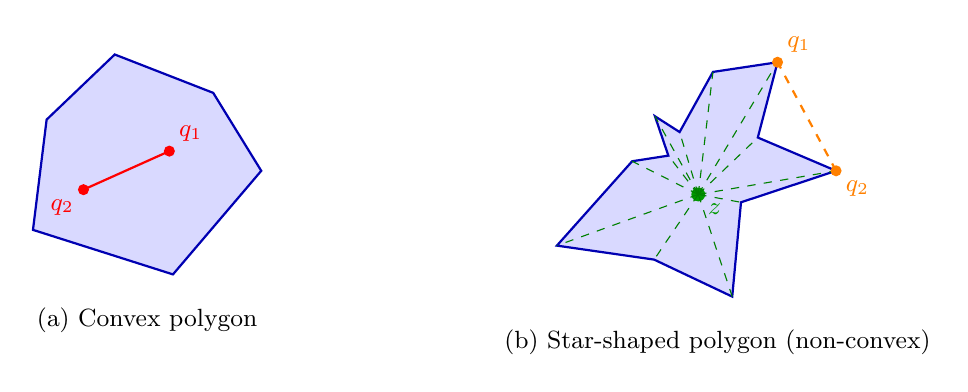
\begin{tikzpicture}
		% Left: Convex polygon
		\begin{scope}[shift={(-3.5,0)}, local bounding box=convex]
			\coordinate (A) at (0:1.6);
			\coordinate (B) at (45:1.4);
			\coordinate (C) at (100:1.5);
			\coordinate (D) at (150:1.3);
			\coordinate (E) at (210:1.5);
			\coordinate (F) at (290:1.4);

			\fill[blue!15] (A) -- (B) -- (C) -- (D) -- (E) -- (F) -- cycle;
			\draw[blue!70!black, thick] (A) -- (B) -- (C) -- (D) -- (E) -- (F) -- cycle;

			\fill[red] (30:0.5)  circle (2pt) node[above right, font=\small] {$q_1$};
			\fill[red] (200:0.7) circle (2pt) node[below left, font=\small]  {$q_2$};
			\draw[red, thick] (30:0.5) -- (200:0.7);

			\node[below, yshift=-0.3cm] at (convex.south) {\small (a) Convex polygon};
		\end{scope}

		% Right: Star-shaped polygon (non-convex, jagged)
		\begin{scope}[shift={(3.5,0)}, local bounding box=starshaped]
			% Jagged star-shaped polygon (irregular, concave indentations on right side)
			\coordinate (S0)  at (  0:1.9);
			\coordinate (S1)  at ( 25:1.0);
			\coordinate (S2)  at ( 50:1.8);
			\coordinate (S3)  at ( 75:1.3);
			\coordinate (S4)  at (100:0.5);
			\coordinate (S5)  at (120:0.8);
			\coordinate (S6)  at (140:0.3);
			\coordinate (S7)  at (170:0.7);
			\coordinate (S8)  at (210:1.9);
			\coordinate (S9)  at (250:1.2);
			\coordinate (S10) at (290:1.7);
			\coordinate (S11) at (330:0.8);

			\fill[blue!15] (S0) -- (S1) -- (S2) -- (S3) -- (S4) -- (S5) -- (S6) -- (S7) -- (S8) -- (S9) -- (S10) -- (S11) -- cycle;
			\draw[blue!70!black, thick] (S0) -- (S1) -- (S2) -- (S3) -- (S4) -- (S5) -- (S6) -- (S7) -- (S8) -- (S9) -- (S10) -- (S11) -- cycle;

			% Kernel point z
			\coordinate (Z) at (0.15, -0.3);
			\fill[green!60!black] (Z) circle (2.5pt) node[below right, font=\small] {$z$};

			% Rays from kernel z to all boundary vertices
			\foreach \i in {0,...,11} {
				\draw[green!50!black, dashed, thin] (Z) -- (S\i);
			}

			% Two interior points whose segment exits the polygon (non-convexity)
			\fill[orange] (S2)  circle (2pt) node[above right, font=\small] {$q_1$};
			\fill[orange] (S0) circle (2pt) node[below right, font=\small] {$q_2$};
			\draw[orange, thick, dashed] (S0) -- (S2);

			\node[below, yshift=-0.3cm] at (starshaped.south) {\small (b) Star-shaped polygon (non-convex)};
		\end{scope}
	\end{tikzpicture}

	\caption{Illustration of convex and star-shaped polygons. (a) A convex polygon: the segment $\overline{q_1 q_2}$ connecting any two interior points lies entirely within the polygon. (b) A star-shaped polygon that is not convex: the kernel point $z$ (near the center) sees all boundary vertices (dashed green), yet the segment $\overline{q_1 q_2}$ connecting two interior points exits the polygon, demonstrating that the interior is not a convex set.}
	\label{fig:geometry-definitions}
\end{figure}

A \textbf{convex polygon} is a polygon whose interior forms a convex set. A polygon $P$ is convex if its interior region is a convex set \cite{preparata1985}. A region $R$ is a convex set if, for any two points $q_1$ and $q_2$ in $R$, the segment $\overline{q_1 q_2}$ is entirely contained in $R$ \cite{preparata1985}. Intuitively, for a convex polygon, the line segment connecting any two points inside the polygon lies entirely within the polygon, and no interior angle exceeds $180^\circ$.

A \textbf{star-shaped polygon} generalizes the notion of convexity. A polygon $P$ is star-shaped if there exists a point $z$ not external to $P$ such that for all points $p$ of $P$, the line segment $\overline{zp}$ lies entirely within $P$ \cite{preparata1985}. The set of all such points $z$ is called the \textit{kernel} of the polygon. A star-shaped polygon can be viewed as one where there is at least one interior point visible to every other point in the polygon. Every convex polygon is star-shaped (the kernel is the entire interior), but a star-shaped polygon may have indentations that make it non-convex.

A \textbf{star-convex polygon} is a polygon $P$ that is simultaneously star-shaped and convex. This dual property makes star-convex polygons particularly useful for representing cell nuclei: because they are convex, every boundary point can be uniquely described by a single ray emanating from the centroid, and because they are star-shaped, the centroid can be placed at a kernel point where all such rays intersect the boundary exactly once. In polar coordinates, a star-convex polygon centered at its centroid $\mathbf{c}$ can therefore be completely represented by a set of radial distances $\{d_0, d_1, \ldots, d_{n-1}\}$ measured at $n$ fixed angular intervals from the centroid to the boundary.

\subsubsection{Suitability for Nuclei Representation}

The star-convex polygon representation is well-suited for representing cell nuclei because of their characteristic morphology. The majority of cell nuclei encountered in H\&E-stained tissue sections are approximately convex or roundish in shape \cite{weigert2022stardist}. Healthy epithelial nuclei are round or elliptical, fibroblasts and endothelial cells are elongated but convex, and even malignant nuclei with pleomorphic variations largely retain a convex silhouette in their two-dimensional projection. This near-ubiquitous convexity means that a star-convex polygon can capture the full boundary geometry of a nucleus with a compact set of radial distances, avoiding the information loss of axis-aligned bounding boxes while remaining far more parameter-efficient than dense per-pixel segmentation masks \cite{schmidt2018cell}.

\subsection{End-to-End Detection with Bipartite Matching}
\label{sec:e2e-matching}

\subsubsection{Bipartite Matching: Hungarian Algorithm}

Bipartite matching establishes a one-to-one correspondence between two sets of elements by finding an optimal assignment that minimizes a total cost. In the context of object detection, bipartite matching assigns each ground-truth object to exactly one prediction and each prediction to at most one ground-truth object, eliminating the ambiguity inherent in IoU-based assignment where multiple predictions can match the same ground-truth object.

The assignment is formulated as a minimum-cost bipartite matching problem. Given a set of $N$ ground-truth objects and $M$ predictions, a cost matrix $\mathbf{C} \in \mathbb{R}^{N \times M}$ is constructed where $C_{i,j}$ measures the dissimilarity between ground-truth $i$ and prediction $j$. A common choice is the negative IoU: $C_{i,j} = 1 - \text{IoU}(g_i, p_j)$. The optimal assignment is found by solving:

\begin{equation}
    \begin{aligned}
        \min_{x_{i,j}} \quad & \sum_{i=1}^{N} \sum_{j=1}^{M} C_{i,j} \, x_{i,j} \\
        \text{s.t.} \quad & \sum_{j=1}^{M} x_{i,j} = 1, \quad \forall i \in \{1, \ldots, N\} \\
        & \sum_{i=1}^{N} x_{i,j} \leq 1, \quad \forall j \in \{1, \ldots, M\} \\
        & x_{i,j} \in \{0, 1\}
    \end{aligned}
\end{equation}

where $x_{i,j} = 1$ if ground-truth $i$ is assigned to prediction $j$, and $0$ otherwise. The first constraint ensures every ground-truth object receives exactly one match. The second constraint ensures no prediction is matched to more than one ground-truth object. When $M > N$, predictions not assigned to any ground-truth are treated as background.

The \textbf{Hungarian algorithm} (Kuhn--Munkres) solves this problem in $O(\max(N, M)^3)$ time through the following steps on a square cost matrix (padded with large values if $N \neq M$): (1) subtract the row minimum from each row, (2) subtract the column minimum from each column, (3) cover all zero entries with the minimum number of horizontal and vertical lines, (4) if the number of lines equals $N$, an optimal assignment is found by selecting independent zeros; otherwise, subtract the smallest uncovered value from all uncovered entries, add it to all doubly covered entries, and repeat from step 3.

This bipartite matching formulation is the foundation of end-to-end detection frameworks such as DETR. By guaranteeing a unique assignment, it eliminates the need for NMS as a post-processing step, since each ground-truth object is matched to exactly one prediction and there are no duplicate assignments to suppress.

\subsubsection{Task-Aligned Matching}
\label{sec:tal}

Task-aligned matching is an assignment strategy used in YOLO-based detection frameworks that jointly considers classification and localization quality when matching predictions to ground-truth objects. Rather than using IoU alone, task-aligned matching defines a combined alignment metric:

\begin{equation}
	t = s^{\alpha} \cdot u^{\beta}
\end{equation}

where $s$ is the classification confidence score, $u$ is the predicted IoU between the prediction and the ground-truth object, and $\alpha, \beta$ are weighting hyperparameters that balance the contribution of classification and localization. A prediction is assigned to a ground-truth object only if its alignment metric $t$ exceeds a threshold, and each ground-truth object is assigned to the prediction with the highest $t$ value. This ensures that predictions assigned to an object are both well-localized (high IoU) and confidently classified, improving training stability.

\subsubsection{Dual-Label Assignment}
\label{sec:dual-label}

Dual-label assignment, introduced in YOLO26, is a training strategy that combines one-to-many and one-to-one matching within a single architecture to achieve the benefits of both paradigms. The model employs two parallel detection heads: a \textbf{one-to-many head} that assigns multiple predictions to each ground-truth object (as in conventional YOLO training), and a \textbf{one-to-one head} that enforces a unique bipartite matching between predictions and ground-truth objects (as in DETR-style training).

The two heads are balanced through an \textbf{annealing weight schedule} that controls their relative contribution to the total loss. During early training epochs, the one-to-many head dominates, providing dense gradient signals that stabilize training and accelerate feature learning. As training progresses, the weight shifts gradually toward the one-to-one head, which refines the predictions to produce unambiguous, duplicate-free detections. This transition allows the model to benefit from the richer supervision of one-to-many matching early on while converging to the cleaner one-to-one assignment necessary for NMS-free inference. At inference time, only the one-to-one head is used, eliminating the need for non-maximum suppression.

\subsection{Evaluation Metrics}

\subsubsection{Precision, Recall, and F1 Score}

Object detection and segmentation are evaluated by comparing predicted instances against ground-truth annotations. Each prediction is classified as a \textbf{true positive (TP)} if it correctly matches a ground-truth object, a \textbf{false positive (FP)} if it does not correspond to any ground-truth object, or a \textbf{false negative (FN)} if a ground-truth object is missed. The definition of a correct match depends on the task: for bounding-box or polygon-based detection, a prediction is typically considered a TP if its intersection over union (IoU) with the ground truth exceeds a threshold $\tau$ (commonly $\tau = 0.5$); for centroid-based detection, a prediction may be considered a TP if the distance between the predicted and ground-truth centroids falls below a distance threshold.

Given the counts of TP, FP, and FN, precision and recall are defined as:

\begin{equation}
    \text{Precision} = \frac{TP}{TP + FP}, \qquad
    \text{Recall}    = \frac{TP}{TP + FN}
\end{equation}

Precision measures the fraction of predictions that are correct (fewer FPs yield higher precision), while recall measures the fraction of ground-truth objects that are found (fewer FNs yield higher recall). The two are often in tension: a model that predicts conservatively achieves high precision but low recall, while a model that predicts aggressively achieves high recall but low precision.

The \textbf{F1 score} is the harmonic mean of precision and recall, providing a single balanced metric:

\begin{equation}
    F1 = \frac{2 \cdot \text{Precision} \cdot \text{Recall}}{\text{Precision} + \text{Recall}}
\end{equation}

\subsubsection{Mean Average Precision (mAP)}

Mean Average Precision (mAP) is the standard evaluation metric for object detection. It is computed by first calculating precision--recall curves for each object class and then averaging the area under these curves across all classes.

Given a set of detections ranked by confidence score and a chosen match criterion (typically $\text{IoU} > 0.5$), precision and recall are computed at each confidence threshold to produce a precision--recall curve. The Average Precision (AP) for a single class is then the area under the interpolated precision--recall curve:

\begin{equation}
	\text{AP} = \int_0^1 P_{\text{interp}}(R) \, dR
\end{equation}

where $P_{\text{interp}}(R) = \max_{\tilde{R} \geq R} P(\tilde{R})$ is the interpolated precision at recall level $R$. In practice, this is approximated by evaluating precision at a discrete set of recall points.

The mean Average Precision is then the mean of per-class AP values:

\begin{equation}
	\text{mAP} = \frac{1}{C} \sum_{c=1}^{C} \text{AP}_c
\end{equation}

where $C$ is the number of object classes. When reported at a specific IoU threshold (e.g., mAP@0.5), detections are matched using that threshold. The COCO evaluation protocol averages mAP over multiple IoU thresholds:

\begin{equation}
    \text{mAP@[.50:.05:.95]} = \frac{1}{K} \sum_{k=1}^{K} \text{mAP}(\theta_k)
\end{equation}

where $\theta_k \in \{0.50, 0.55, \ldots, 0.95\}$ and $K = 10$. This provides a more comprehensive assessment of localization accuracy than evaluation at a single threshold. The notation $\text{mAP}@0.50$ (or $\text{AP}_{50}$) refers to evaluation at a single IoU threshold of 0.50.

\subsubsection{Panoptic Quality (PQ)}

Panoptic Quality (PQ) was introduced by Kirillov et al.~\cite{kirillov2019panoptic} as a unified metric for panoptic segmentation, combining both recognition quality (detection accuracy) and segmentation quality (boundary accuracy). PQ has become the standard evaluation metric for nuclei instance segmentation benchmarks such as PanNuke~\cite{gamper2020pannuke} and CoNIC~\cite{graham2021conic}.

Given a ground truth segmentation $G$ and a predicted segmentation $P$, each instance in $G$ and $P$ is uniquely labeled. A predicted segment $\hat{s}$ is matched to a ground truth segment $s$ if and only if their intersection over union (IoU) exceeds a threshold, typically $\text{IoU} > 0.5$:

\begin{equation}
	\text{IoU}(s, \hat{s}) = \frac{|s \cap \hat{s}|}{|s \cup \hat{s}|}
\end{equation}

After matching, PQ is computed as:

\begin{equation}
	\text{PQ} = \underbrace{\frac{|TP|}{|TP| + \frac{1}{2}|FP| + \frac{1}{2}|FN|}}_{\text{Recognition Quality (RQ)}} \times \underbrace{\frac{\sum_{(s,\hat{s}) \in TP} \text{IoU}(s, \hat{s})}{|TP|}}_{\text{Segmentation Quality (SQ)}}
\end{equation}

where $TP$ is the set of true positive pairs (matched ground truth--prediction pairs), $FP$ is the set of false positive predictions (unmatched predictions), and $FN$ is the set of false negative ground truth segments (unmatched ground truth). PQ thus decomposes into two interpretable components:

\begin{itemize}
	\item \textbf{Recognition Quality (RQ):} measures detection accuracy and is equivalent to the F1 score computed over matched and unmatched segments.
	\item \textbf{Segmentation Quality (SQ):} measures the average IoU of correctly matched pairs, quantifying how precisely the predicted boundaries align with the ground truth.
\end{itemize}

Several PQ variants are commonly reported in nuclei segmentation literature:

\begin{itemize}
	\item \textbf{Instance PQ (iPQ):} evaluates PQ on a per-image basis and then averages across all images in the dataset. Each image contributes equally regardless of the number of nuclei it contains.
	\item \textbf{Multi-class PQ (mPQ):} extends PQ to multi-class settings by computing PQ independently for each nuclei type and then averaging across all classes:
	\begin{equation}
		\text{mPQ} = \frac{1}{C} \sum_{c=1}^{C} \text{PQ}_c
	\end{equation}
	where $C$ is the number of classes and $\text{PQ}_c$ is the PQ computed for class $c$ only.
	\item \textbf{Binary PQ (bPQ):} computes PQ in a binary setting where all nuclei types are treated as a single class, ignoring type-specific distinctions. This is useful for evaluating pure instance segmentation performance independent of classification accuracy.
	\item \textbf{PanNuke PQ (nuPQ):} the specific PQ variant used in the PanNuke benchmark, which computes mPQ across the 19 nuclei type categories defined in the dataset.
\end{itemize}

\subsubsection{Aggregated Jaccard Index (AJI)}
\label{sec:aji}

The Aggregated Jaccard Index (AJI) \cite{kumar2017dataset} is an instance-level segmentation metric designed to address the overcounting problem in the standard Jaccard Index when applied to multi-object segmentation. In nuclei segmentation, the standard Jaccard Index (Intersection over Union, IoU) computed per instance and then averaged can overestimate performance because each ground-truth nucleus is free to match with any predicted nucleus independently, and unmatched predictions do not penalize the score.

AJI resolves this by computing a single global intersection-over-union across all instances. Given a set of ground-truth nuclei $G = \{g_1, g_2, \ldots, g_N\}$ and predicted nuclei $P = \{p_1, p_2, \ldots, p_M\}$, AJI first finds the optimal one-to-one assignment that maximizes total pairwise IoU. Let $\mathcal{M} \subseteq G \times P$ denote the set of matched pairs, $G_{\text{matched}} \subseteq G$ the set of matched ground-truth nuclei, and $P_{\text{matched}} \subseteq P$ the set of matched predicted nuclei. The AJI is then defined as:

\begin{equation}
    \text{AJI} = \frac{\displaystyle\sum_{(g_i, p_j) \in \mathcal{M}} |g_i \cap p_j|}{\displaystyle\sum_{(g_i, p_j) \in \mathcal{M}} |g_i \cup p_j| + \sum_{g_k \in G \setminus G_{\text{matched}}} |g_k| + \sum_{p_l \in P \setminus P_{\text{matched}}} |p_l|}
\end{equation}

The numerator sums the intersection area over all matched pairs, while the denominator sums the union area over all matched pairs plus the areas of all unmatched ground-truth and predicted nuclei. This formulation penalizes both false negatives (unmatched ground-truth nuclei) and false positives (unmatched predictions), providing a more stringent evaluation than per-instance averaging.
